\chapter{Process-Partitioned Coloured~Petri~Nets}
\label{chap:netclass}
%\begin{itemize}
%\item motivation: why do we need this class, what does it capture 
%\item net class explained through the producer-consumer example.
%\item formel def. 
%\item Intuitiv forklaring af netklassen
%\item Formel definition
%\end{itemize}

A general Coloured Petri Net is not limited to regular control flow structures in the same way common programming languages are. For this reason it is not easy to capture the behaviour of a CPN model by using common programming constructs, e.g., sequences, loops, and case-statements. Because of this, a restricted class of CPNs is needed in order to be able to automatically generate code from a CPN model. In this section we present a subclass of CPNs called \emph{Process-Partitioned Coloured Petri Nets} (ProPCPNs or ProPCP-nets). ProPCP-nets are restricted in such a way that it is possible to recognise structures that can be translated into common programming language constructers. The definition of ProPCP-nets is inspired by the definition made by Kristensen and Valmari in \cite{RefWorks:82}.

The main property of ProPCP-nets is that they are partitioned into separate processes. This means that process partitions can be executed in parallel without influencing the behaviour of each other except for some synchronisation points. Another important property of ProPCP-nets is that each process partition has the control flow of the process explicitly represented in the structure of the net. This has the consequence that the state of the model always reflects where in the control flow the process is. Furthermore, access to stored values local to each process partition, is also represented explicitly in the model to be able to determine the local state of the process.

Section~\ref{sec:cpnformal} presents the formal definition of CP-nets along with some concepts concerning the semantics. In section \ref{sec:netclassinformal} we introduce and motivate ProPCP-nets by showing how the CPN model of the producer-consumer system fits into this class of CPN models. Then, in section \ref{sec:netclassformal}, the class of ProPCP-nets is summarised in a formal definition.


\section{The Formal Definition of CP-nets}
\label{sec:cpnformal}
In order to understand the definition of ProPCP-nets we first present definition \ref{def:cpnet} which is the same as definition 4.2 given in (p. 91, \cite{RefWorks:87}). It defines the syntax of a Coloured Petri Net which is the net structure, the types, the variables and the net inscriptions of the CP-net.

\newtheorem{definition}{Definition}
\begin{definition}
\label{def:cpnet}
A \defconcept{Coloured Petri Net} is a nine-tuple \\ $\mathit{CPN} =
(P,T,A,\Sigma,V,C,G,E,I)$ where:

\begin{enumerate}

\item $P$ is a finite set of \defconceptmodindex{places}{place}.

\item $T$ is a finite set of \defconceptmodindex{transitions}{transition} $T$ such that $P \cap T = \emptyset$.

\item $A \subseteq P \times T \cup T \times P$ is a set of directed \defconceptmodindex{arcs}{arc}.

\item $\Sigma$ is a finite set of non-empty \defconceptmodindex{colour sets}{colour set}. 

\item $V$ is a finite set of \defconceptmodindex{typed variables}{typed variable} such that $\mathit{Type}[v] \in \Sigma$ for all variables $v \in V$.

\item $C : P \rightarrow \Sigma$ is a \defconcept{colour set function} assigning a colour set to each place.

\item $G : T \rightarrow \mathit{EXPR}_V$ is a \defconcept{guard function} 
assigning a guard to each transition $t$ such that $\mathit{Type}[G(t)] = \mathit{Bool}$.

\item $E : A \rightarrow \mathit{EXPR}_V$ is an \defconcept{arc expression function} assigning an arc expression to each arc $a$ such that $\mathit{Type}[E(a)] = C(p)_{MS}$, where $p$ is the place connected to the arc $a$.

\item $I : P \rightarrow \mathit{EXPR}_{\emptyset}$ is an
\defconcept{initialisation function} assigning an initialisation
expression to each place $p$ such that $\mathit{Type}[I(p)] =
C(p)_{MS}$.

\end{enumerate}
\flushright $\square$
\end{definition}

\noindent
Definition \ref{def:semanticconcepts} is a part of definition 4.3 given in (p. 93, \cite{RefWorks:87}) with definition 3.a added. It defines some concepts concerning the semantics of the CP-net.

\begin{definition}
\label{def:semanticconcepts}

For a CP-net $\mathit{CPN} = (P,T,A,\Sigma,V,C,G,E,I)$ we define the following concepts:

\begin{enumerate}

\item[1.] A \defconcept{marking} is a function $M$ mapping each place
$p$ into a multi-set of tokens $M(p) \in C(p)_{MS}$.

\item[2.] The \defconcept{initial marking} $M_0$ is defined by $M_0(p)
= I(p)\langle \rangle$ for all $p \in P$.

\item[3.] The \defconceptmodindex{variables of a transition}{variables of transition} $t$ is denoted
$\mathit{Var}(t) \subseteq V$ and consists of the free variables appearing in
the guard of $t$ or in the arc expressions of arcs connected to $t$.

\begin{enumerate}
\item[a.] The \defconceptmodindex{variables of an expression}{variables of an expression} $e$ is denoted $\mathit{Var}(e) \subseteq V$ and consists of the free variables appearing in $e$.
\end{enumerate}

\item[4.] A \defconcept{binding} of a transition $t$ is a function $b$
mapping each variable $v \in \mathit{Var}(t)$ into a value $b(v) \in
\mathit{Type}[v]$.
%The set of all bindings for a transition $t$ is denoted $B(t)$.

\item[5.] A \defconcept{binding element} is a pair $(t,b)$ such that
$t \in T$ and $b \in B(t)$. The set of all binding elements
$\mathit{BE}(t)$ for a transition $t$ is defined by $\mathit{BE}(t) =
\{ (t,b) \; | \; b \in B(t) \}$. The set of all binding elements in a
CPN model is denoted $\mathit{BE}$.

%\item[6.] A \defconcept{step} $Y \in BE_{MS}$ is a non-empty and finite multi-set of binding elements.  

\end{enumerate}
\flushright $\square$
\end{definition}
\section{The Producer-Consumer System as a ProPCPN}
\label{sec:netclassinformal}
A model belonging to ProPCPN is divided into \emph{process partitions}. The CPN model of the producer-consumer system presented in section~\ref{sec:cpn} belongs to the class of ProPCP-nets. We introduce the ProPCPN by explaining what makes the producer-consumer system as a ProPCPN model. The model of the producer-consumer system shown in Fig.~\ref{fig:netclasssystem} is the same as Fig.~\ref{fig:systemmodule} in section~\ref{sec:cpn} except that the objects in this model are painted with colours to show their type. Buffer places are painted blue, shared places are painted red, and local places are painted green. To symbolise the control flow we use a thick black line around process places, transitions, and process arcs.

\begin{figure}[b!]
\centering
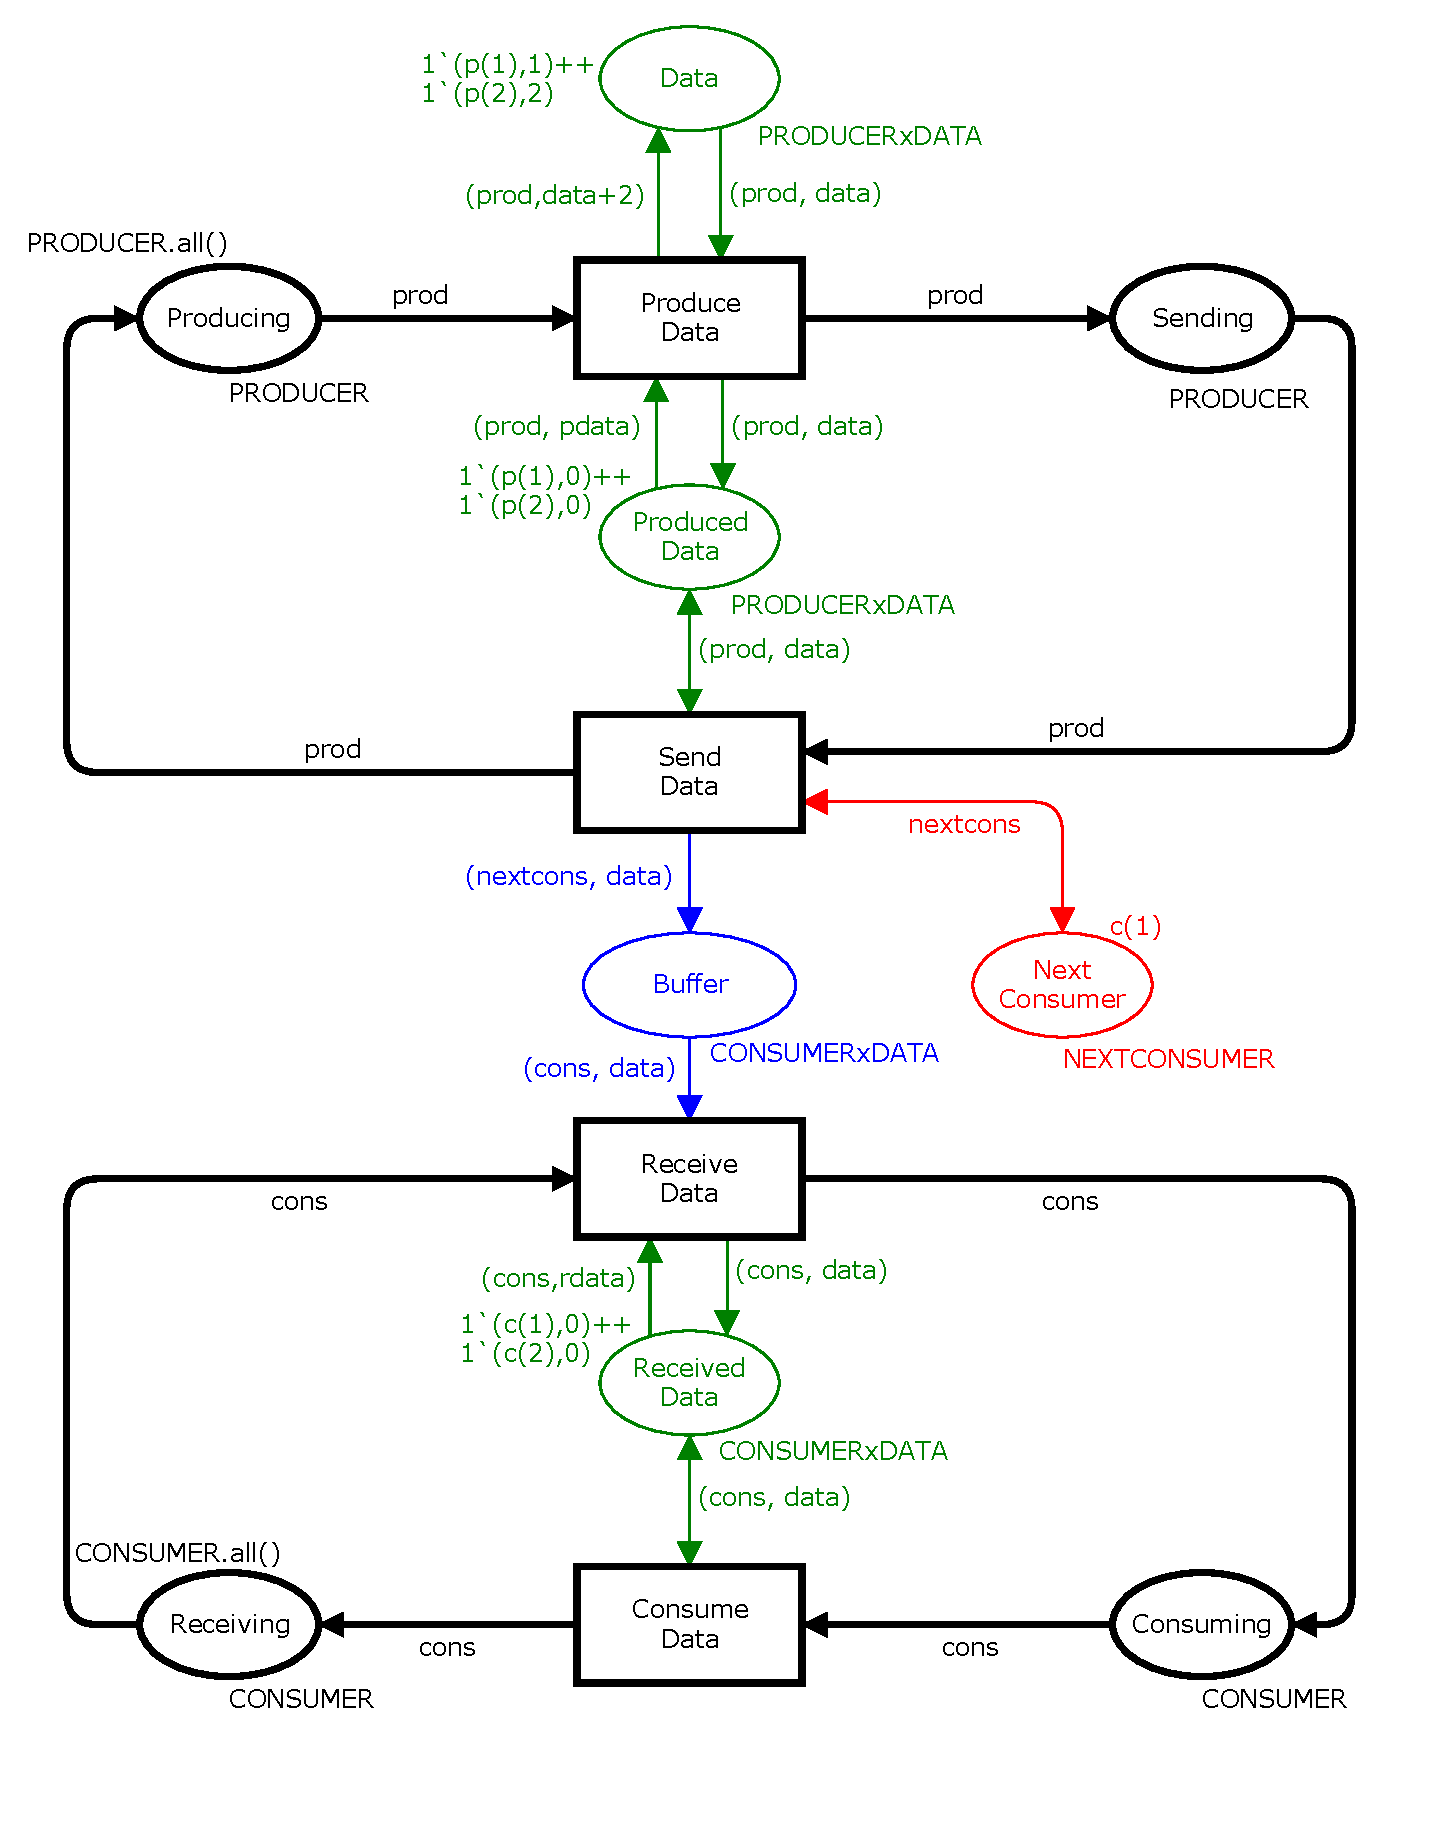
\includegraphics[scale=0.5]{netclass/graphics/System.eps}
\caption{The producer-consumer system with two process partitions}
\label{fig:netclasssystem}
\end{figure}

The model has two process partitions, one modelling the producers (top) and a one modelling the consumers (bottom). Process partitions can be connected by either \emph{buffer} or \emph{shared} places, but are otherwise disjoint. In Fig.~\ref{fig:netclasssystem} the producer and consumer are only connected by the buffer place \figitem{Buffer}. Intuitively, a process partition models the state and actions of one or more \emph{process instances} running the same program code. In the producer-consumer system the producer process partition models two producer process instances running the same program code. Transitions in a ProPCP-net belong to a unique process partition, e.g., the transition \figitem{SendData} in Fig.~\ref{fig:netclasssystem} belongs to the producer process partition.

\subsection{The Places of a ProPCP-net}
There are four types of places in ProPCP-nets:\! \emph{process places}, \emph{local places}, \emph{buffer places} and \emph{shared places}. The set of all places in the ProPCPN is denoted $P$. $P_{pro} \subseteq P$ denotes the set of process places, $P_{loc} \subseteq P$ denotes the set of local places, $P_{buf} \subseteq P$ denotes the set of buffer places, and $P_{sha} \subseteq P$ denotes the set of shared places. These sets are disjoint and together they constitute all places in the ProPCPN, i.e., $P = P_{pro} \uplus P_{loc} \uplus P_{buf} \uplus P_{sha}$. In the producer-consumer system the places are divided into:

\begin{center}
\begin{tabular}{l c l}
$P_{pro}$ & = & \{\figitem{\,Producing}, \figitem{Sending}, \figitem{Receiving}, \figitem{Consuming}\,\}\\
$P_{loc}$ & = & \{\figitem{\,Data}, \figitem{ProducedData}, \figitem{ReceivedData}\,\}\\
$P_{buf}$ & = & \{\figitem{\,Buffer}\,\}\\
$P_{sha}$ & = & \{\figitem{\,NextConsumer}\,\}
\end{tabular}
\end{center}

\noindent
The colour sets in a ProPCPN can be described as follows $\Sigma = \Sigma_{P} \uplus \Sigma_{D} \uplus \Sigma_{C}$, where $\Sigma_{C} = \Sigma_{P} \times \Sigma_{D}$. $\Sigma_{P}$ contains the process types and $\Sigma_{D}$ contains data types which can be any colour set not contained in $\Sigma_{P}$ or $\Sigma_{C}$. In the producer-consumer system the sets contains the following colour sets:

\begin{center}
\begin{tabular}{l c l}
$\Sigma_{P}$ & = & \{\code{\,PRODUCER}, \code{CONSUMER\,}\}\\
$\Sigma_{D}$ & = & \{\code{\,DATA\,}\}\\
$\Sigma_{C}$ & = & \{\code{\,PRODUCERxDATA}, \code{CONSUMERxDATA\,}\}
\end{tabular}
\end{center}

\subsubsection{Process Places}

\begin{figure}
\centering
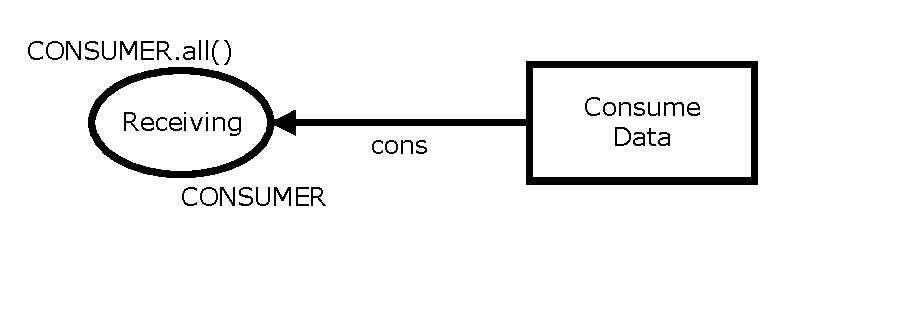
\includegraphics[scale=0.5]{netclass/graphics/process_place.eps}
\caption{The process place \figitem{Receiving} in the \code{consumer} process partition}
\label{fig:processplace}
\end{figure}

The control flow of a process is modelled using \emph{process places}. In the producer-consumer system (see Fig.~\ref{fig:netclasssystem}) the places \figitem{Producing} and \figitem{Sending} are process places in the producer process partition, and \figitem{Receiving} and \figitem{Consuming} are process places in the consumer process partition. The colour set of a process place is required to be a process type, i.e., $C(p) \in \Sigma_{P}$ for $p \in P_{pro}$. A token residing on a process place is called a \emph{process token} and the colour of the token identifies the corresponding process instance. Taking a closer look at the process place \figitem{Receiving} in the consumer process partition (shown in Fig.~\ref{fig:processplace}) we see that is has the colour set \code{CONSUMER} declared as:

\begin{verbatim}
colset CONSUMER = index c with 1..2 declare pid;
\end{verbatim} 

\noindent
This means that the only tokens which can reside on a process place in the consumer process partition is the tokens \code{c(1)} and \code{c(2)}, which corresponds to the two consumer process instances. Notice that the declaration has \code{declare pid} attached to it which defines this colour set to be a process type. In general, the colour set of a process place must have the form:

\begin{verbatim}
colset PROCESS = index p with 1..n declare pid;
\end{verbatim}

\noindent
where \code{PROCESS} is the name of the process partition, \code{p} is the process partition identifier and the integer \code{n} specifies the number of process instances of the process partition.

In every reachable marking a process token must reside on exactly one process place of the partition. This is because a process instance cannot be in two different positions in the control flow at the same time. For instance, the consumer process token \code{c(1)} cannot reside on both the process place \figitem{Receiving} and \figitem{Consuming}. This dynamic property is ensured by imposing the static restriction that every transition must be connected to exactly one input process place and exactly one output process place. Taking a look at the transition \figitem{ConsumeData} in Fig.~\ref{fig:consumedatatrans} we see that it has the input process place \figitem{Consuming} and the output process place \figitem{Receiving}. Formally, this property is expressed as:

\begin{displaymath}
\begin{array}{l}
\text{for all } t \in T: \mid \{ (p, t) \mid p \in P_{pro}, (p, t) \in A \}\mid = 1 \text{ and, } \\
\text{for all } t \in T: \mid \{ (t, p) \mid p \in P_{pro}, (t, p) \in A \}\mid = 1 
\end{array}
\end{displaymath}

\begin{figure}
\centering
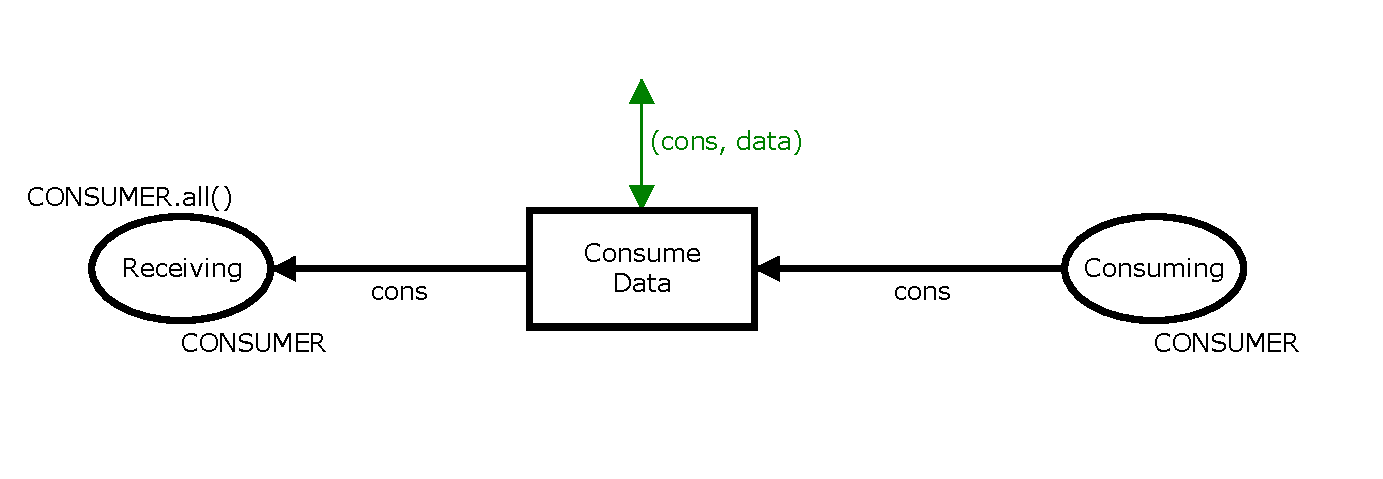
\includegraphics[scale=0.5]{netclass/graphics/consumedatatrans.eps}
\caption{The transition \figitem{ConsumeData} in the \code{consumer} process partition}
\label{fig:consumedatatrans}
\end{figure}

\noindent
The arc expressions on the input and output arcs to a process place is simply a process variable. Thus, when a binding element containing the transition \figitem{ConsumeData} occurs it removes a process token from \figitem{Consuming} and adds a token to \figitem{Receiving}. In the general case, it is imposed that an occurrence of a binding element removes exactly one process token from the input process places, and adds exactly one process token to the output process place. Also it must be the same process token being removed and added, i.e., the process token is in the same colour set and has the same index value. To express this formally we first define $C_{T}: T \rightarrow \Sigma_{P}$ to be the function that maps each transition to a unique process type. This process type is the same as the type of the process tokens which the transitions move. For the producer-consumer system the function is defined as:

\begin{displaymath}
C_{T}(t) = \left\{ 
\begin{array}{ll}
\code{PRODUCER} & \mbox{ if }  t \in \{\,\figitem{ProduceData}, \figitem{SendData}\,\} \\
\code{CONSUMER} & \mbox{ if }  t \in \{\,\figitem{ReceiveData}, \figitem{ConsumeData}\,\}
\end{array}\right.
\end{displaymath}

\noindent
The requirement that every transition must consume a token from a process place and add a token to a process place can now be expressed as follows: for all $t \in T$ it is the case that for $p_{1}, p_{2} \in P_{pro}$ where $(t, p_{1}) \in A$ and $(p_{2}, t) \in A$ it holds that $E(t, p_{1}) = E(p_{2}, t) = v \in V$ and $C_{T}(t) = Type[v]$.

The initial marking of a process place intuitively represents the starting point for a process instance. All process instances within a process partition must start at the same point in the control flow. This means that in the initial marking there is one process place containing all process token in each process partition. The table below shows the initial marking of the process places in the producer-consumer system.

\begin{center}
\begin{tabular}{| c | c |}
\hline
\textbf{Process place} & \textbf{Initial marking}\\
\hline
\figitem{Producing} & \code{PRODUCER.all()}\\ 
\hline
\figitem{Receiving} & \code{CONSUMER.all()} \\
\hline
\figitem{Sending}, \figitem{Consuming} & $\msempty$ \\
\hline
\end{tabular}
\end{center}

\noindent
The colour set function \code{all()} returns a multi-set containing one token of each colour in the colour set. The process place \figitem{Producing} contains all the process tokens of the \code{PRODUCER} process partition, and the process place \figitem{Receiving} contains all the process tokens of the \code{CONSUMER} process partition. No other process places contain any tokens in the initial marking. Formally, we define this requirement as follows: For all $\sigma \in \Sigma_{P} $ it is the case that:

\begin{equation}
\label{processsum}
\sum_{p \in P_{pro}, C(p) = \sigma} I(p)\langle \rangle = \sigma
\end{equation}

\noindent
and there exists a place:
\begin{equation}
\label{placeexists}
p \in P_{pro} \text{ where } I(p)\langle \rangle = \sigma
\end{equation}

\noindent
Equation \eqref{processsum} ensures that all tokens of a given process type reside on some place in the initial marking. Equation \eqref{placeexists} ensures that there exists a place where all process tokens of a given process type resides in the initial marking. Jointly, they ensure that all process tokens of a given type reside on exactly one place in the initial marking.

\subsubsection{Local Places}

\begin{figure}
\centering
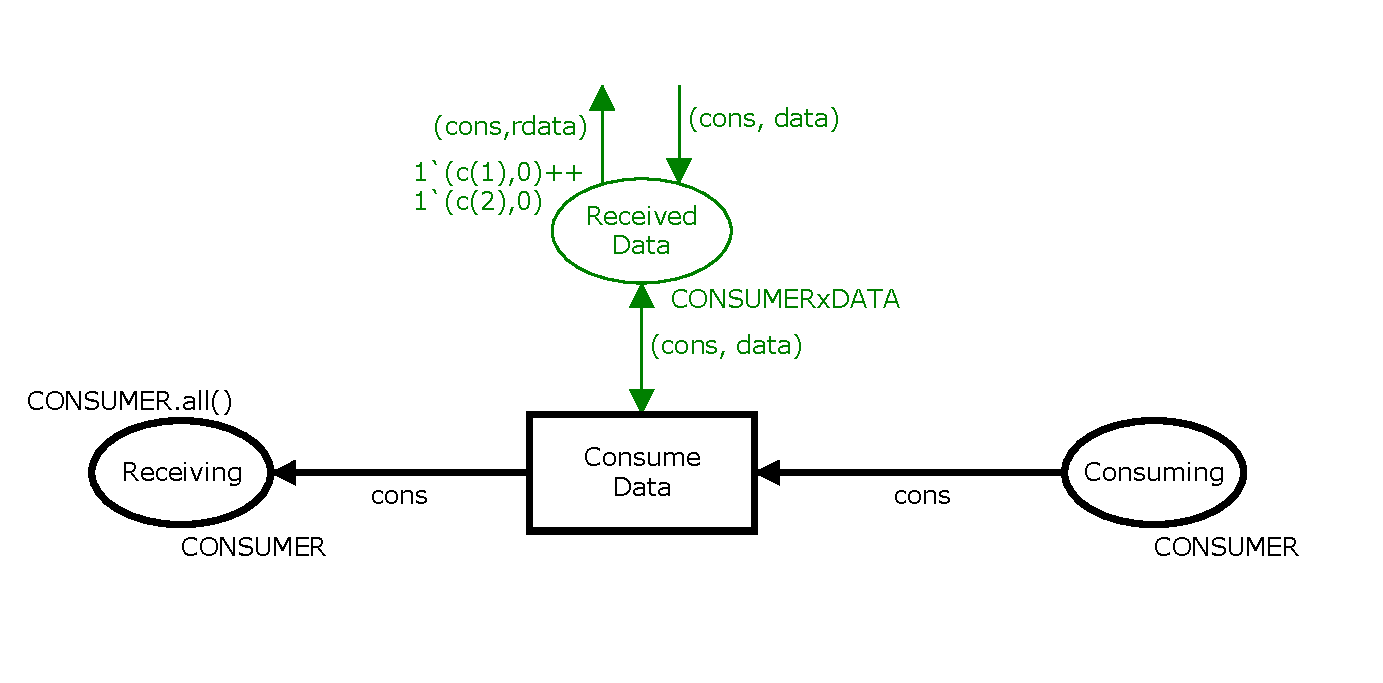
\includegraphics[scale=0.45]{netclass/graphics/local_place.eps}
\caption{The local place \figitem{ReceivedData} in the consumer process partition}
\label{fig:localplace}
\end{figure}

Local places are used to store data local to a process. A token residing on a local place is private to a specific process instance, thus local places can be used to keep data only visible within a process instance. This concept is very similar to variables in computer programs. In the producer-consumer system we have three local places: \figitem{Data}, \figitem{ProducedData} and \figitem{ReceivedData}. A local place is required to have a product colour set consisting of a process type and some data type, e.g., 

\begin{verbatim}
colset CONSUMERxDATA = product CONSUMER * DATA;
\end{verbatim} 

\noindent
This is the colour set of the local place \figitem{ReceivedData} shown in Fig.~\ref{fig:localplace}. In this case \code{DATA} is an integer, but it could be an arbitrary colour set in $\Sigma_{C}$, i.e., it is the case that $C(p) \in \Sigma_{C}$ for $p \in P_{loc}$. Notice, that the two input arcs to the transition \figitem{ConsumeData} ensures that the process token removed from \figitem{Consuming} is the same as the process token in the \code{CONSUMERxDATA} pair removed from the local place \figitem{ReceivedData}.

For a given transition \emph{t} and a local place \emph{p} we require that: If there is an input arc from \emph{p} to \emph{t}, there also has to be an output arc going from \emph{t} to \emph{p}, and the other way around, i.e.,

\begin{displaymath}
\text{For all } t \in T \text{ and for all } p \in P_{loc} : (p, t) \in A \Leftrightarrow (t, p) \in A
\end{displaymath}

\noindent
This assures that a local place always contains exactly one pair per process instance. For the same reason the initial marking of a local place has to contain one pair for each process instance. If we look at a local place $p \in P_{loc}$ with colour set $C(p) = C_{P} \times C_{D}$ the initial marking of that place contains exactly one token per process instance, i.e., $I(p)\langle \rangle_{1} = C_{P}$ where $I(p)\langle \rangle_{1}$ is the projection of the product colour set onto the first component.

%$\mid I(p)\langle \rangle \mid = \mid C_{P} \mid$ and for all $c_{P} \in C_{P}$ there must exist a $c_{D} \in C_{D}$ such that $(c_{P}, c_{D}) \in I(p)\langle \rangle$.

In order to express requirements on arc expression we define $V_{T}: T \rightarrow V$ to be the function that maps each transition to a unique process variable which is the variable found on arcs between process places and transitions. This process variable has the same type as the transition, i.e., for all $t \in T$ : $Type[V_{T}(t)] = C_{T}(t)$. In the producer-consumer system this function is defined as:

\begin{displaymath}
V_{T}(t) = \left\{ 
\begin{array}{ll}
\code{prod} & \mbox{ if }  t \in \{\,\figitem{ProduceData}, \figitem{SendData}\,\} \\
\code{cons} & \mbox{ if }  t \in \{\,\figitem{ReceiveData}, \figitem{ConsumeData}\,\}
\end{array}\right.
\end{displaymath}

\noindent
The arc expression on an outgoing arc from a local place $p$ to a transition $t$ is restricted to the form: \code{(process, data)} where \code{process} is a variable of type \code{PROCESS} and \code{data} is a variable of type \code{DATA}. This can be expressed as: $E(p, t) = (V_{T}(t), v_{D}) \in V \times V$. The expression on an arc from a transition $t$ to a local place $p$ is restricted to the form: \code{(process, expr)} where \code{process} is the same process variable as on the outgoing arc, and the type of the result from evaluating \code{expr} is \code{DATA}. Formally this is: $E(t, p) = (V_{T}(t), e)$ where $e$ is any expression.

%Finally, it is only allowed for a transition $t$ to add tokens to or remove tokens from a local place $p$ belonging to its own process partition. Formally put, let $C(p) = C_{P} \times C_{D}$ for $p \in P_{loc}$ and $(p, t) \in A$. Then $C_{P} = C_{T}(t)$.

\subsubsection{Buffer Places}

\begin{figure}[b!]
\centering
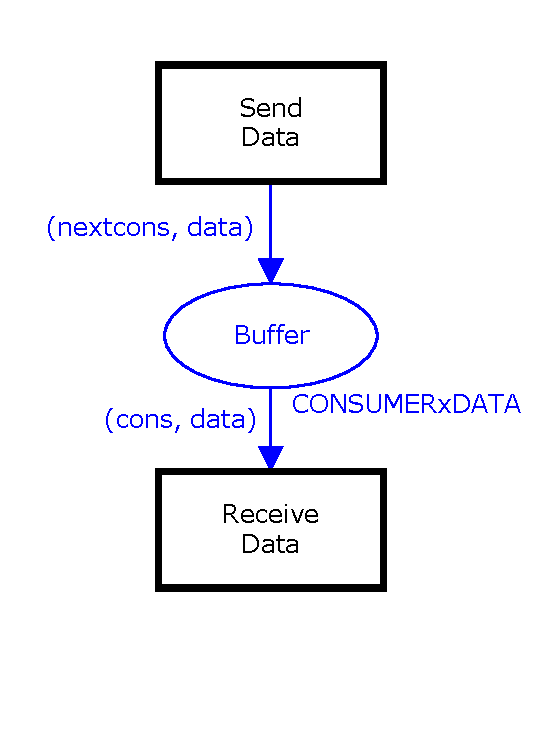
\includegraphics[scale=0.45]{netclass/graphics/buffer_place.eps}
\caption{The buffer place \figitem{Buffer} in the producer-consumer model}
\label{fig:bufferplace}
\end{figure}
%Buffer places and shared places are used to model asynchronous communication between processes, including communication between processes within the same process partition. They are the only ways to connect different process partitions.

Buffer places can be used to send data directly to a process instance. Unlike local places there can be zero or more tokens on a buffer place. Intuitively, a buffer place is a buffer local to a specific process instance in which received data from other processes is put. This can be thought of as a communication channel which allows process to communicate in an asynchronous way. The producer-consumer model has one buffer place named \figitem{Buffer} which can be seen in Fig.~\ref{fig:bufferplace}. The colour set of a buffer place $p$ is (as for local place) a pair consisting of a process variable and some data, i.e., $C(p) \in \Sigma_{C}$. 

The initial marking of a buffer place is required to be the empty multi-set, i.e., for all $p \in P_{buf}$ it holds that $I(p)\langle \rangle = \msempty$. There can be zero or more input arcs to a buffer place and zero or more output arcs from a buffer place. In the producer-consumer system, the buffer place \figitem{Buffer} has one input arc from the transition \figitem{SendData} and one output arc to the transition \figitem{ReceiveData} (see Fig.~\ref{fig:bufferplace}). This way \figitem{Buffer} connects the \code{producer} process partition to the \code{consumer} process partition. 

Arc expressions on outgoing arcs from buffer places are restricted to the form: \code{(process, data)} where \code{process} is the process variable of type \code{PROCESS} and \code{data} is a variable of type \code{DATA}. Formally, this is defined as:

\begin{displaymath}
\text{For all } p \in P_{buf} \text{ it holds that } E(p, t) = (V_{T}(t), v_{d}) \in V \times V
\end{displaymath}

\noindent
The arc expression on an incoming arc to a buffer place has no restrictions since the type of the process variable does not have to be that same as \code{process} in the pair \code{(process, expr)} (like it was the case for local places).

\subsubsection{Shared Places}

\begin{figure}
\centering
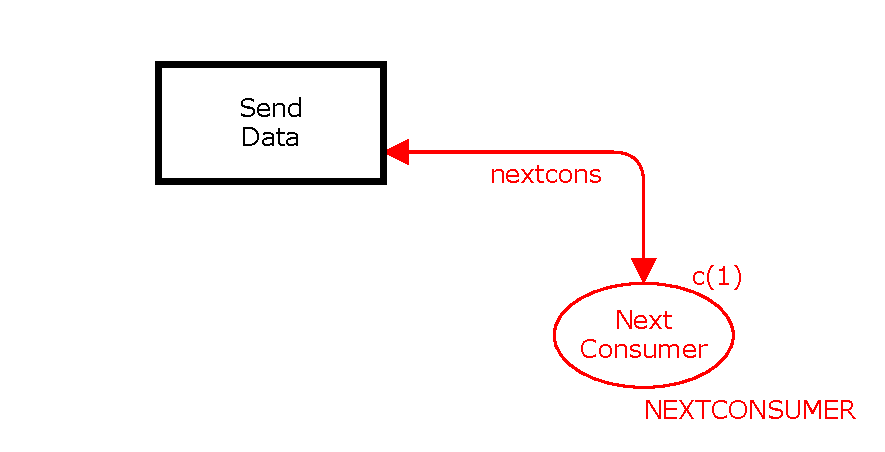
\includegraphics[scale=0.45]{netclass/graphics/shared_place.eps}
\caption{The shared place \figitem{NextConsumer} in the producer-consumer model}
\label{fig:sharedplace}
\end{figure}

Shared places can be used to share data between several processes. Intuitively, a shared place is a global variable which can be written to and read from by all process instances. In the producer-consumer system \figitem{NextConsumer} (shown in Fig.~\ref{fig:sharedplace}) is a shared place. The colour set of a shared place can be any type in $\Sigma_{D}$, i.e., $C(p) \in \Sigma_{D}$ for $p \in P_{sha}$. The initial marking of a shared place is required to have exactly one token, i.e., for all $p \in P_{sha}$ it holds that $\mid I(p)\langle \rangle \mid = 1$.

For the transition \figitem{SendData} there is both an input arc from, and an output arc to, the shared place \figitem{NextConsumer} (in this case a double arc). This must be true in general, i.e., for a given transition \emph{t} and a shared place \emph{p}: if there is an input arc from \emph{p} to \emph{t}, we require that there is an output arc going from \emph{t} to \emph{p}. Formally, this is defined as:

\begin{displaymath}
\text{For all } p \in P_{sha} \text{ it is the case that } (p, t) \in A \Leftrightarrow (t, p) \in A
\end{displaymath}

\noindent
Along with the restriction on bindings (defined below), this is ensures the there always is one token on a shared place.

%The arc expression on an outgoing arc from a shared place with colour set \code{DATA} must have the form \code{data}, where data is a variable with type \code{DATA}, and the arc expression on an incoming arc must have the form \code{expr}, where \code{expr} evaluate to something of type \code{DATA}.

\subsection{Variables and Bindings}
To ensure that the "flow of tokens" is preserved through the execution of the model all bindings of arc expressions are required to evaluate to a multi-set containing exactly one token. Intuitively, we can say that each arc either consumes or produces exactly one token. Therefore, we require that:

\begin{displaymath}
\begin{array}{l}
\text{For all } (p, t), (t, p) \in A \text{ and for all } b \in BE(t) \text{ it is the case:} \\
\mid E(p, t)\langle b \rangle \mid = \mid E(t, p)\langle b \rangle \mid = 1
\end{array}
\end{displaymath}

\noindent
Except for process variables, a variable is not allowed to reside on more than one input arc to a transition. Having the same variable on, e.g., two input arcs from two different local places would mean that the transition is only enabled when the values on the two local places are equal. We express this as:

\begin{displaymath}
\begin{array}{l}
\text{For all } t \in T \text{ and for } p_{1}, p_{2} \in P \text{ where } p_{1} \neq p_{2} \text{ it holds:} \\
Var(E(p_{1}, t)) \cap Var(E(p_{2}, t)) \subseteq \{V_{T}(t)\}
\end{array}
\end{displaymath}

\noindent
Ensuring that two variables have the same value can still be achieved in a ProPCP-net by having the equality check in the guard for that transition.

Free variables are not allowed on output arcs or in guard expressions. We ensure this restriction of output arc expressions by requiring that the set of variables on an output arc from a transition is a subset of the set of variables on all input arcs: For all $t \in T$ it is the case that for all $(t, p) \in A$:

\begin{equation*}
Var(E(t, p)) \subseteq \bigcup_{(p^{\prime}, t) \in A} Var(E(p^{\prime}, t))
\end{equation*}

Variables in a guard expression for a transition must be variables found on input arcs from local places, i.e., guard expressions are not allowed to contain variables read from buffer, shared or process places. Furthermore, guards must not contain free variables . This can be expressed as: for all $t \in T$ it holds that $G(t) \in EXPR_{V^{\prime}}$ where

\begin{equation*}
V^{\prime} = \bigcup_{p \in P_{loc}, (p, t) \in A} Var(E(p, t)) \setminus {V_{T}(t)}
\end{equation*}

\section{The Formal Definition of ProPCP-nets}
\label{sec:netclassformal}
This section summarises the formal definition of the syntax of the ProPCPN modelling language presented above. We define two functions associating transitions with a process partition:

\begin{enumerate}
\item $C_{T} : T \rightarrow \Sigma_{P}$ \textit{maps each transition to a unique process colour set.}
\item $V_{T} : T \rightarrow V$ \textit{maps each transition to a unique process variable where for all} $t \in T$ : $Type[V_{T}(t)] = C_{T}(t)$
\end{enumerate}

\noindent
These functions are used in definition~\ref{def:propcpn} which summarises the definition of ProPCP-net from section~\ref{sec:netclassinformal}:

% ProPCPN
\begin{definition}
\label{def:propcpn}
A \defconcept{Process-Partitioned Coloured Petri Net} is a Coloured Petri Net $\mathit{CPN} =
(P,T,A,\Sigma,V,C,G,E,I)$, where:

\begin{enumerate}
%% TYPES
\item $\Sigma = \Sigma_{P} \uplus \Sigma_{D} \uplus \Sigma_{C}$, where $\Sigma_{C} = \{\sigma_{p} \times \sigma_{d} \mid \sigma_{p} \in \Sigma_{P}, \sigma_{d} \in \Sigma_{D}\}$.

%% PLACE TYPES
\item $P = P_{pro} \uplus P_{loc} \uplus P_{buf} \uplus P_{sha}$

\begin{enumerate}
\item $C(p) \in \Sigma_{P}$ for $p \in P_{pro}$
\item $C(p) \in \Sigma_{D}$ for $p \in P_{sha}$
\item $C(p) \in \Sigma_{C}$ for $p \in P_{loc} \cup P_{buf}$
\end{enumerate}

%% LOCAL PLACES
\item Let $p \in P_{loc}$ and $C(p) = C_{P} \times C_{D}$:

\begin{enumerate}
\item $(p, t) \in A \Leftrightarrow (t, p) \in A$
%\item $(p, t) \in A \Rightarrow C_{P} = C_{T}(t)$
\item $E(p, t) = (V_{T}(t), v_{D}) \in V \times V$
\item $E(t, p) = (V_{T}(t), e)$ where $e$ is an expression%$e \in EXPR_{C_{D}}$.
\end{enumerate}

\item For all $p \in P_{buf}$ : $E(p, t) = (V_{T}(t), v_{d}) \in V \times V$.

\item For all $p \in P_{sha}$ : $(p, t) \in A \Leftrightarrow (t, p) \in A$.
%\\
%\\
%\textbf{Initial markings}
%%% INITIAL MARKINGS
%\item For all $\sigma \in \Sigma_{P} $ :
%\begin{equation*}
%\mssum_{p \in P_{pro}, C(p) = \sigma} I(p)\langle \rangle = \sigma
%\end{equation*}
%and there exists a place $p \in P_{pro}$ where $I(p)\langle \rangle = \sigma$
%
%\item For all $p \in P_{loc}$ where $C(p) = C_{P} \times C_{D}$ : $\mid I(p)\langle \rangle \mid = \mid C_{P} \mid$ and for all $c_{p} \in C_{P}$ there exists $c_{D} \in C_{D}$ such that $(c_{P}, c_{D}) \in I(p)\langle \rangle$.
%\item For all $p \in P_{buf}$ : $I(p)\langle \rangle = \emptyset$
%\item For all $p \in P_{sha}$ : $\mid I(p)\langle \rangle \mid = 1$
%\\
%\\
%\textbf{Transitions}
%%% TRANSITIONER
%%\item For all $t \in T$ there exists $p \in P_{pro}$ such that $(p, t) \in A$ and $(t, p) \in A$.
%
%\item For all $t \in T$ : $\mid \{ (p, t) \mid p \in P_{pro}, (p, t) \in A \}\mid = \mid \{ (t, p) \mid p \in P_{pro}, (t, p) \in A \}\mid = 1$
%
%\item For all $t \in T$ there exists exactly one $p_{1} \in P_{pro}$ and exactly one $p_{2} \in P_{pro}$ where $(t, p_{1}) \in A$ and $(p_{2}, t) \in A$ : $E(t, p_{1}) = E(p_{2}, t) = v \in V$ and $C_{T}(t) = Type[v]$.
%\\
%\\
%\textbf{Bindings and variables}
%% BINDINGS
\item For all $(p, t), (t, p) \in A$ and for all $b \in BE(t)$ :\\
$\mid E(p, t)\langle b \rangle \mid = \mid E(t, p)\langle b \rangle \mid = 1$

%% GUARDS
\item For all $t \in T$ : $G(t) \in EXPR_{V^{\prime}}$ where

\begin{equation*}
V^{\prime} = \bigcup_{p \in P_{loc}, (p, t) \in A} Var(E(p, t)) \setminus {V_{T}(t)}
\end{equation*}

%% VARIABLES
\item For all $t \in T$ and for $p_{1}, p_{2} \in P$ where $p_{1} \neq p_{2}$ :\\
$Var(E(p_{1}, t)) \cap Var(E(p_{2}, t)) \subseteq \{V_{T}(t)\}$

\item For all $t \in T$ : for all $(t, p) \in A$.

\begin{equation*}
Var(E(t, p)) \subseteq \bigcup_{(p^{\prime}, t) \in A} Var(E(p^{\prime}, t))
\end{equation*}

\item The initial marking is process initialising. (See definition \ref{def:processinit})
\item All transitions are flow preserving. (See definition \ref{def:flowpreserving})

\end{enumerate}
\flushright $\square$
\end{definition}

\noindent
The enabling and occurrence of steps in a ProPCP-net is the same as for general CP-nets, i.e., ProPCP-nets follows the definition of semantics in general CP-nets and the concepts defined in definition~\ref{def:semanticconcepts}. Next, we define the concept of an initial marking being process initialising.

\begin{definition}
\label{def:processinit}
For an initial marking to be \defconcept{process initialising} it must hold that:

\begin{enumerate}
\item For all $\sigma \in \Sigma_{P} $ :
\begin{equation*}
\mssum_{p \in P_{pro}, C(p) = \sigma} I(p)\langle \rangle = \sigma
\end{equation*}
and there exists a place $p \in P_{pro}$ where $I(p)\langle \rangle = \sigma$

%\item For all $p \in P_{loc}$ where $C(p) = C_{P} \times C_{D}$ : $\mid I(p)\langle \rangle \mid = \mid C_{P} \mid$ and for all $c_{p} \in C_{P}$ there exists $c_{D} \in C_{D}$ such that $(c_{P}, c_{D}) \in I(p)\langle \rangle$.

\item For all $p \in P_{loc}$ : $I(p)\langle \rangle_{1} = C_{P}$
\item For all $p \in P_{buf}$ : $I(p)\langle \rangle = \emptyset$
\item For all $p \in P_{sha}$ : $\mid I(p)\langle \rangle \mid = 1$
\end{enumerate}
\flushright $\square$
\end{definition}

\noindent
Finally, in definition \ref{def:flowpreserving} we define the concept of a transition being flow preserving.

\begin{definition}
\label{def:flowpreserving}
For a transition to be \defconcept{flow preserving} it must hold that:

\begin{enumerate}
\item For $t \in T$ :\\
$\mid \{ (p, t) \mid p \in P_{pro}, (p, t) \in A \}\mid = \mid \{ (t, p) \mid p \in P_{pro}, (t, p) \in A \}\mid = 1$

%\item For $t \in T$ there exists exactly one $p_{1} \in P_{pro}$ and exactly one $p_{2} \in P_{pro}$ where $(t, p_{1}) \in A$ and $(p_{2}, t) \in A$ : $E(t, p_{1}) = E(p_{2}, t) = v \in V$ and $C_{T}(t) = Type[v]$.

\item For all $t \in T$, $p_{1}, p_{2} \in P_{pro}$ where $(t, p_{1}) \in A$ and $(p_{2}, t) \in A$ : $E(t, p_{1}) = E(p_{2}, t) = v \in V$ and $C_{T}(t) = Type[v]$.

\end{enumerate}
\flushright $\square$
\end{definition}

